\lecture{Лекция 11}{lec11}
\subtitle{Лекция 11 --- Программирование: Рекурсия}

\frame[plain]
{\titlepage}	% Титульный слайд


\begin{frame}
\frametitle{Программирование}

\begin{center}

\Huge
Понятие рекурсии
\end{center}
\end{frame}

	\begin{frame}
\frametitle{Понятие рекурсии}
Алгоритм принято называть рекурсивным, если в его определении содержится прямой или косвенный вызов этого же алгоритма. 

Вычисления, проводимые с помощью рекурсивных алгоритмов (процедур, функций) называют рекурсивными. 
Различают два базовых вида рекурсии: \textbf{прямая} и \textbf{косвенная}. 

\end{frame}

		\begin{frame}
\frametitle{Понятие рекурсии}


Под \textbf{прямой} рекурсией принято понимать непосредственный вызов алгоритма (функции, процедуры) F из текста самого алгоритма F. 

При \textbf{косвенной} рекурсии мы имеем циклическую последовательность вызовов нескольких алгоритмов $F_1, F_2, …, F_k$ (функций, процедур) друг друга: $F_1$ вызывает $F_2$, $F_2$ вызывает $F_3$, $\ldots$, $F_k$ вызывает $F_1$ $(k>1)$.


\end{frame}

		\begin{frame}
\frametitle{Рекурсивная триада}

А.Р Есаяном предложена схема решения задач с помощью рекурсии, основным компонентом которой является рекурсивная триада, состоящая из трех базовых этапов: 
\begin{enumerate}
	\item параметризация, 
	\item выделение базы (или выделение начальной базы и правил её изменения), 
	\item декомпозиция.
\end{enumerate}

\end{frame}

		\begin{frame}
\frametitle{Параметризация}

Параметризация задачи заключается в выявлении совокупности исходных величин, определяющих постановку и решение задачи. 

Значения этих параметров или некоторых из них влияют на трудоемкость решения задачи. 

Иногда бывает полезно ввести в рассмотрение дополнительные параметры, напрямую с постановкой задачи не связанные, но помогающие организовать рекурсию.

\end{frame}

		\begin{frame}
\frametitle{Выделение базы}

Выделение базы --- поиск одной или нескольких подзадач, которые бывают решены непосредственно без рекурсивного вызова. В случае если база будет меняться в процессе вычислений, то должен быть указан алгоритм её изменения. 

Как правило, подобная динамическая база расширяется за счет получения решений промежуточных задач и облегчает выполнение процесса отложенных вычислений. Возможно и сужение рекурсивной базы.

\end{frame}

		\begin{frame}
\frametitle{Декомпозиция}

Декомпозиция общего случая --- это процесс последовательного разложения задачи на серию подзадач двух типов: тех, которые мы решать умеем и тех, которые в чем-то аналогичны исходной задаче. 

В последнем случае каждая из полученных подзадач должна быть упрощенным вариантом предыдущей задачи. При этом декомпозицию следует осуществлять так, чтобы можно было доказать, что при любом допустимом наборе значений параметров рано или поздно она приведет нас к одному из выделенных тривиальных случаев, то есть к базе.

\end{frame}

\begin{frame}
\frametitle{Пример: Факториал}


\begin{enumerate}
	\item Параметризация: $n$ --- число, факториал которого ищем
	\item Выделение базы: $1!=1$, $0!=1$.
	\item Декомпозиция: $n!=n\cdot(n-1)!$
\end{enumerate}


\end{frame}

\begin{frame}
\frametitle{Пример: Факториал}
\setlength{\columnsep}{-7cm}
\begin{multicols}{2}
\lstinputlisting[style=CStyle]{prg/factorial.pas}
Запись 3 (->2) означает, что номер рекурсивного вызова 3, номер возврата 2.
\columnbreak
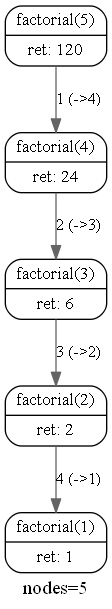
\includegraphics[height=7.5cm, right]{images/factorial.png}
\end{multicols}

\end{frame}


\begin{frame}[fragile]
\frametitle{Пример: Числа Фибоначчи}

Числа Фибоначчи --- элементы числовой последовательности
\begin{verbatim}
0, 1, 1, 2, 3, 5, 8, 13, 21, 34, 55, 89, 144, 233, 377, 610,... 
(последовательность A000045 в OEIS)
\end{verbatim}
    
в которой первые два числа равны либо 1 и 1, либо 0 и 1, а каждое последующее число равно сумме двух предыдущих чисел. Названы в честь средневекового математика Леонардо Пизанского (известного как Фибоначчи). 
\begin{enumerate}
	\item Параметризация: $n$ --- номер числа, Фибоначчи
	\item Выделение базы: $f_1=1$, $f_2=1$.
	\item Декомпозиция: $f_n=f_{n-1}+f_{n-2}$
\end{enumerate}

\end{frame}


\begin{frame}
\frametitle{Пример: Числа Фибоначчи}
\setlength{\columnsep}{-7cm}
\begin{multicols}{2}


\lstinputlisting[style=CStyle]{prg/fib.pas}

\columnbreak

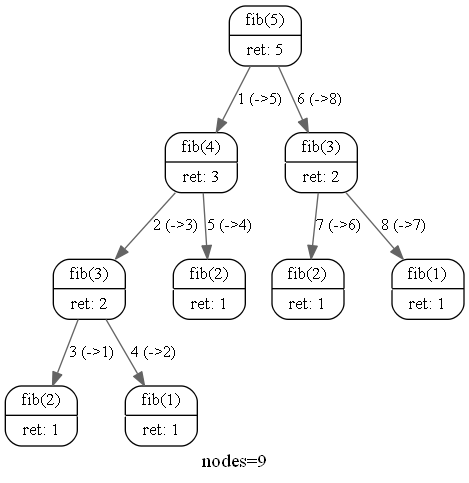
\includegraphics[height=7cm, right]{images/fib.png}

\end{multicols}

\end{frame}


\begin{frame}
\frametitle{Программирование}

\begin{center}

\Huge
Примеры решения задач
\end{center}
\end{frame}

\begin{frame}[fragile]
\frametitle{Пример 1}

Ниже записана рекурсивная процедура:
\begin{lstlisting}[style=CStyle]
procedure F(n: integer);
begin
  if n > 1 then begin
    F(n - 4);
    write(n);
    F(n div 2);
  end;
end;
\end{lstlisting}
Что будет напечатано на экране при выполнении вызова F(11)?

\end{frame}

\begin{frame}[fragile]
\frametitle{Пример 1: Дерево рекурсивных вызовов}

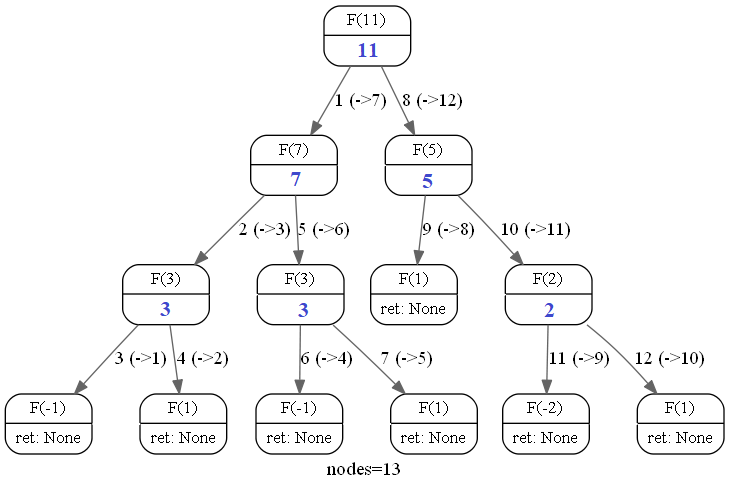
\includegraphics[height=8cm, center]{images/rec01.png}
\end{frame}

\begin{frame}[fragile]
\frametitle{Пример 1: Дерево рекурсивных вызовов}

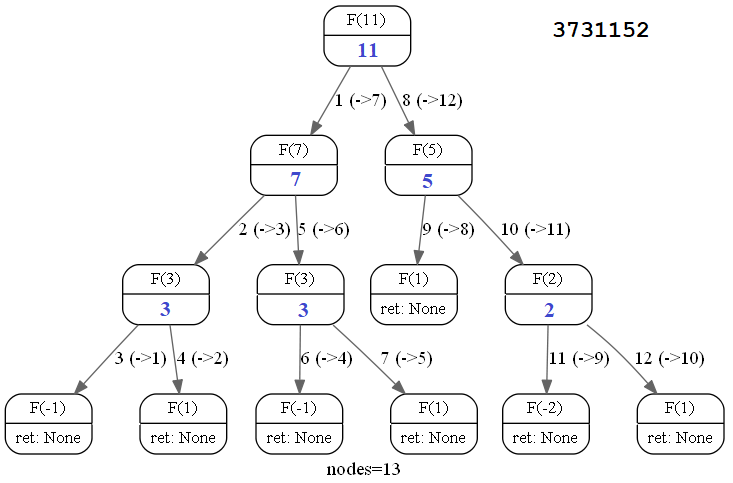
\includegraphics[height=8cm, center]{images/rec011.png}
\end{frame}

\begin{frame}[fragile]
\frametitle{Пример 2}

Дан рекурсивный алгоритм:
\begin{lstlisting}[style=CStyle]
procedure F(n: integer);
begin
  writeln(n);
  if n < 5 then begin
    F(n + 1);
    F(n + 3)
  end
end;

\end{lstlisting}
Найдите сумму чисел, которые будут выведены при вызове F(1).

\end{frame}

\begin{frame}[fragile]
\frametitle{Пример 2: Дерево рекурсивных вызовов}

\setlength{\columnsep}{-2cm}
\begin{multicols}{2}
Протокол рекурсивных \\вызовов
\small
\begin{verbatim}
F(1), writeln(1) вызов 1
F(2), writeln(2) вызов 2
F(3), writeln(3) вызов 3
F(4), writeln(4) вызов 4
F(5), writeln(5) вызов 5
F(7), writeln(7) вызов 5
F(6), writeln(6) вызов 4
F(5), writeln(5) вызов 3
F(4), writeln(4) вызов 2
F(5), writeln(5) вызов 3
F(7), writeln(7) вызов 3
\end{verbatim}

Ответ 49


\columnbreak

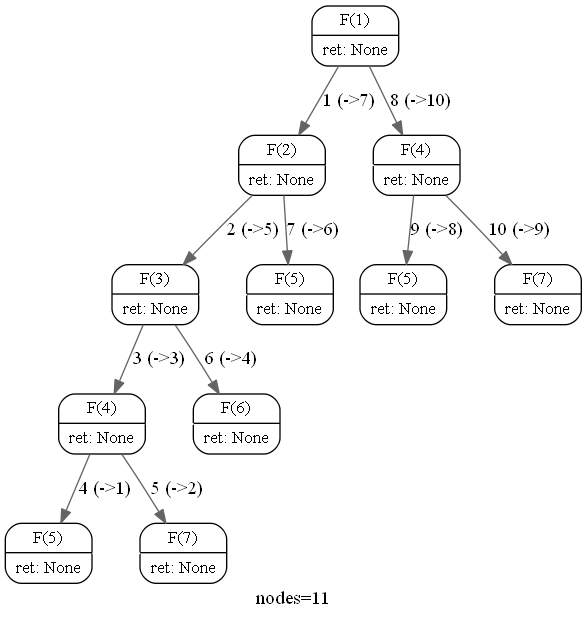
\includegraphics[height=7cm, left]{images/rec02.png}

\end{multicols}


\end{frame}

\begin{frame}[fragile]
\frametitle{Пример 3}

Дан рекурсивный алгоритм:
\begin{lstlisting}[style=CStyle]
procedure F(n: integer);
begin
 writeln('*');
 if n > 0 then begin
   F(n-2);
   F(n div 2)
 end
end;
\end{lstlisting}
Сколько символов <<звездочка>> будет напечатано на экране при выполнении вызова F(7)?

\end{frame}


\begin{frame}[fragile]
\frametitle{Пример 3: Дерево рекурсивных вызовов}

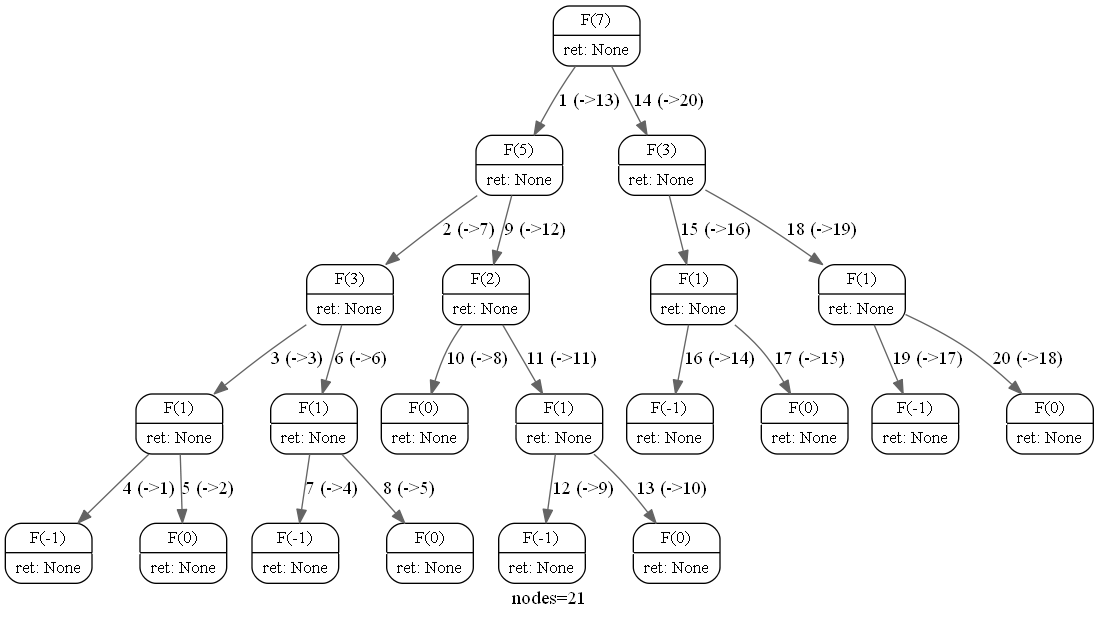
\includegraphics[height=6.5cm, left]{images/rec03.png}
\pause Ответ: 21
\end{frame}


\begin{frame}[fragile]
\frametitle{Пример 4}

Процедура F(n), где n – натуральное число, задана следующим образом (язык Паскаль):
\begin{lstlisting}[style=CStyle]
procedure F(n: integer);
begin
  if n < 3 then
    write('*')
  else begin
    F(n-1);
    F(n-2);
    F(n-2)
  end;
end;
\end{lstlisting}
Сколько звездочек напечатает эта процедура при вызове F(6)? В ответе запишите только целое число.

\end{frame}

\begin{frame}[fragile]
\frametitle{Пример 4: Дерево рекурсивных вызовов}
F(6)=F(5)+F(4)+F(4)\\
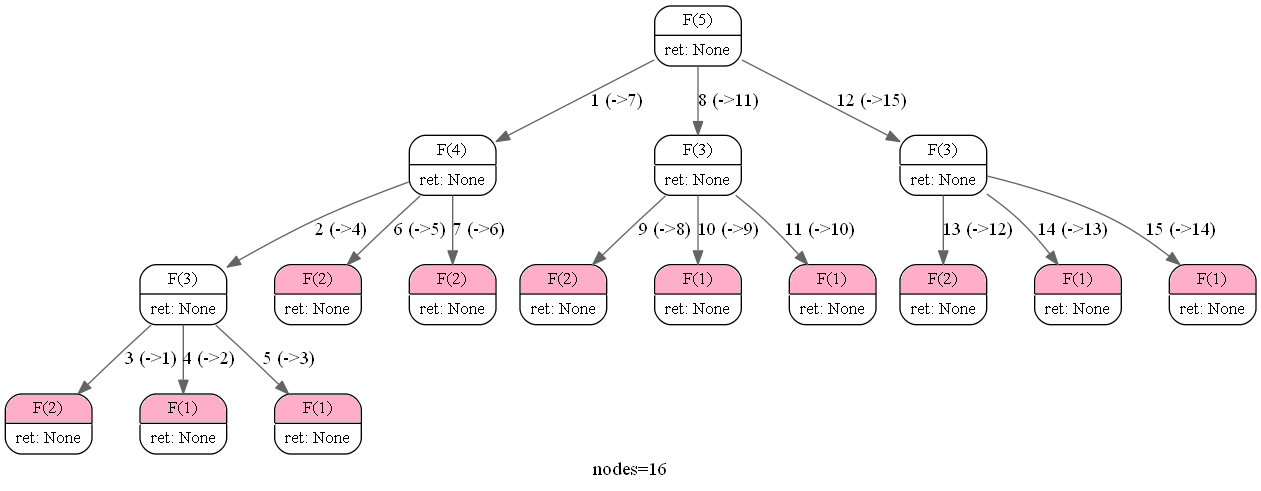
\includegraphics[width=12cm, center]{images/rec04.png}
\end{frame}

\begin{frame}[fragile]
\frametitle{Пример 4: Дерево рекурсивных вызовов}
F(6)=F(5)+F(4)+F(4)\\
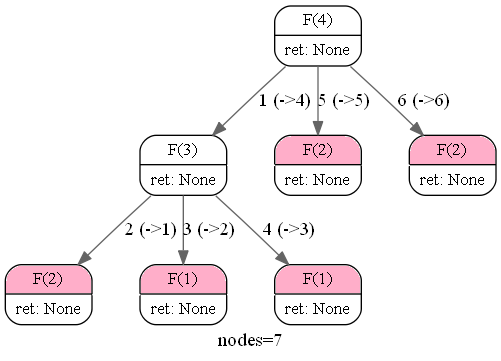
\includegraphics[height=6.5cm, center]{images/rec041.png}
\pause Ответ: 21
\end{frame}